%META {"title":"Cặp góc trong cùng phía bù nhau","note":"Hai góc được đánh dấu nằm cùng phía của đường thẳng c và trong khoảng giữa a, b; tổng của chúng bằng 180° (115° + 65°) → a // b. HS trả lời miệng: hai góc trong cùng phía bù nhau thì hai đường thẳng song song."}
\documentclass[border=5pt]{standalone}
\usepackage{tkz-euclide}
% Màu dùng chung cho toàn bộ hình vẽ (ảnh stack với nền tối của web)
\definecolor{tminc}{RGB}{226,232,240}   % chữ + nét chính
\definecolor{tmblue}{RGB}{0,210,255}    % nhấn neon xanh
\definecolor{tmpink}{RGB}{255,0,200}    % nhấn neon hồng
\definecolor{tmgreen}{RGB}{0,255,136}   % nhấn neon xanh lá
\color{tminc}

\begin{document}
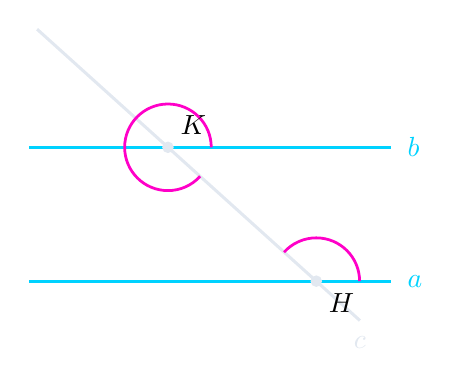
\begin{tikzpicture}[line width=1.1pt]
  \coordinate (A) at (-0.6,0);
  \coordinate (B) at (4,0);
  \coordinate (C) at (-0.6,1.7);
  \coordinate (D) at (4,1.7);
  \coordinate (E) at (-0.5,3.2);
  \coordinate (F) at (3.6,-0.5);
  \tkzInterLL(A,B)(E,F) \tkzGetPoint{P}
  \tkzInterLL(C,D)(E,F) \tkzGetPoint{Q}
  \draw[tmblue] (A) -- (B) node[right=2pt]{$a$};
  \draw[tmblue] (C) -- (D) node[right=2pt]{$b$};
  \draw[tminc] (E) -- (F) node[below=2pt]{$c$};
  \tkzMarkAngles[size=0.55,arc=l,color=tmpink,line width=1pt](B,P,Q)
  \tkzMarkAngles[size=0.55,arc=l,color=tmpink,line width=1pt](D,Q,P)
  \tkzDrawPoints[size=3,color=tminc,fill=tminc](P,Q)
  \tkzLabelPoint[below right=1pt](P){$H$}
  \tkzLabelPoint[above right=1pt](Q){$K$}
\end{tikzpicture}
\end{document}
